% This text is proprietary.
% It's a part of presentation made by myself.
% It may not used commercial.
% The noncommercial use such as private and study is free
% Sep. 2005
% Author: Sascha Frank
% University Freiburg
% www.informatik.uni-freiburg.de/~frank/




\documentclass{beamer}
\usepackage[]{caption}
\setbeamerfont{caption}{size=\fontsize{6}{0}}

\usetheme{Goettingen}

\AtBeginSection[]{
  \begin{frame}
    \vfill
    \centering
    \begin{beamercolorbox}[sep=8pt,center,shadow=true,rounded=true]{title}
      \usebeamerfont{title}\insertsectionhead\par%
    \end{beamercolorbox}
    \vfill
  \end{frame}
}

\begin{document}
\title{Chaos in Seemingly Simple Optical Systems}
\author{Liam Packer}
\date{\today}

\frame{\titlepage}

\frame{\frametitle{Table of contents}\tableofcontents}


\section{A Brief Intro to Nonlinear Optics}
\subsection{Nonlinear Polarization}
\frame{\frametitle{The Linear Polarization}
  \begin{itemize}
  \item In linear optics: $\mathbf{P} \propto \mathbf{E}$
  \item Refractive index $n$ a constant of a material for a given wavelength
  \item Most general, $\mathbf{P} = \epsilon_0\chi^{(1)}(\mathbf{E})$, or $P^i = \epsilon_0\chi_{ij}E^j$
    \begin{figure}[htbp]
      \centerline{\includegraphics[]{polarization.jpg}}
      \caption[]{\label{fig:1} \cite{Polarization} Physical mechanism of (linear) polarization}
    \end{figure}
  \end{itemize}
}

\frame{\frametitle{The Nonlinear Polarization}
  \begin{itemize}
  \item Nonlinear optics idea: Expand $\mathbf{P}$ in iterated products of $\mathbf{E}$
    \begin{align*}
      \mathbf{P} &= \epsilon_0[\chi^{(1)}(\mathbf{E}) + \chi^{(2)}(\mathbf{E}, \mathbf{E}) +
                      \chi^{(3)}(\mathbf{E}, \mathbf{E}, \mathbf{E}) + \cdots]\\
                    &= \mathbf{P}^{(1)} + \mathbf{P}^{(2)} + \mathbf{P}^{(3)} + \cdots\\
      \text{or } P^{i} &= \epsilon_0[\chi^{(1)}_{ij}E^j + \chi^{(2)}_{ijk}E^jE^k +
                         \chi^{(3)}_{ijkl}E^jE^kE^l + \cdots]
    \end{align*}
  \item where $P^{(n)}\equiv \epsilon_0\chi^{(n)}(\mathbf{E}, \mathbf{E}, \cdots)$
  \item (assumes instantaneous response of medium to electric field)
  \end{itemize}
}

\subsection{Intensity-Dependent Refractive Index}
\frame{\frametitle{Intensity-Dependent Refractive Index}
  Lets consider some third-order effects. For simplicity, we'll only work with magnitudes and
  say that $P^{(3)}(t) = \epsilon_0\chi^{(3)}E^3(t) \propto E^3(t)$.
  \begin{itemize}
  \item Picking a monochromatic wave, $E(t) = \mathcal{E}\cos \omega t$
  \item Then, using the identity $\cos^3\omega
    t = \frac14 \cos(3\omega t) + \frac34 \cos \omega t$:
    \[P^{(3)}(t) = \frac14 \epsilon_0\chi^{(3)}\mathcal{E}^3 \cos 3\omega t + \frac34
      \epsilon_0\chi^{(3)}\mathcal{E}^3\cos\omega t\]
  \item Since $n(\omega) = \sqrt{1 + \chi_{eff}(\omega)}$ and $I(\omega) \propto |E(\omega)|^2$, this effects the index of
    refraction: $n(\omega) = n_0 + n_2I(\omega)$ (See Boyd \S 6.2, 2008).
  \end{itemize}
}
\subsection{A Simple System}
\frame{\frametitle{A Simple System}

  \begin{figure}[htbp]
    \centerline{\includegraphics[scale=0.5]{ring-resonator.png}}
    \caption[]{\label{fig:2} \cite{ikeda_optical_1980}}
  \end{figure}
}

\frame{\frametitle{A Simple System (intuition, guesses)}
  \begin{columns}
    % col1
    \begin{column}{0.5\textwidth}
      \begin{itemize}
      \item Linear case: constant phase shift $\phi_0 = \frac{2\pi L}{\lambda}n_0$
      \item Nonlinear case: variable phase shift $\phi(\omega) = \frac{2\pi L}{\lambda} n(\omega)$
      \item Third-order effects: $n(\omega) = n_0 + n_2 I(\omega)$
      \item Equation of motion guess: $\dot{E}(t) \propto E(t) \exp(i \phi)$
      \end{itemize}
    \end{column}

    % col2
    \begin{column} {0.5\textwidth}
      \begin{figure}[htbp]
        \centerline{\includegraphics[scale=0.28]{ring-resonator.png}}
        \caption[]{\label{fig:2} \cite{ikeda_optical_1980}}
      \end{figure}

    \end{column}

  \end{columns}
}

\section{Analysis}
\subsection{The Driving Equations}
\frame{\frametitle{The Driving Equations (complex amplitude)}
  \begin{align}
    \label{eq:1}
    \dot{E}(t) &= A + BE(t - t_R)\exp\{i[\phi(t) - \phi_0]\},\\
    \gamma^{-1}\dot{\phi}(t) &= -\phi(t) + \text{sgn}(n_2)|E(t - t_R)|^2.
  \end{align} \cite{ikeda_optical_1980}
  \begin{itemize}
  \item $E(t) \equiv$ dimensionless (complex) field amplitude at top-left corner of ring
  \item $\phi(t) \equiv$ time-dependent phase shift of the electric field
  \item $A \propto \sqrt{(2\pi/\lambda)n_{2}}E_{in}$, $B\propto
    \sqrt{(2\pi/\lambda)n_2}\hat{E}(t,0)$ a dissipation parameter
  \item $t_R \equiv$ time delay due to propagation of light through cavity
  \item $\phi_0\equiv (2\pi/\lambda) n_0$
  \end{itemize}
}

\frame{\frametitle{The Driving Equations (intensity map)}
  \begin{align}
    \label{eq:1}
    I_{n+1} = I_{in}\bigg(1 + C\cos\big(\frac{2\pi L}{\lambda}(n_0 + n_{2}I_{n})\big)\bigg)
  \end{align}\cite{harrison_chaos_1986}
  \begin{itemize}
  \item $I_n \equiv$ Intensity of electric field at start of $n^{th}$ round trip

  \item $I_{in}\equiv$ Intensity of input electric field
  \item $n_0\equiv$ linear index of refraction, $n_2 \equiv $ second-order index of refraction
  \item $L \equiv$ length of cavity, $\lambda \equiv$ wavelength of monochromatic input light
  \end{itemize}
}


\subsection{Non-Chaotic Regime}
\frame{\frametitle{Non-Chaotic Regime}
  \begin{figure}[htbp]
    \centerline{\includegraphics[scale=0.5]{map-stable.png}}
    \caption[]{\label{fig:3} }
  \end{figure}
}

\subsection{The Road to Chaos}
\frame{\frametitle{The Road to Chaos}

  \begin{columns}
    \begin{column}{0.5\textwidth}
      \begin{figure}[htbp]
        \centerline{\includegraphics[scale=0.25]{map-stable.png}}
        \caption[scale=0.1]{$\lambda\approx -0.3205$, $f'(x_i)\approx 0.72575$\\\qquad\quad$\lambda\approx -0.10966$, $f'(x_i)\approx 0.64491$}
      \end{figure}

      \begin{figure}[htbp]
        \centerline{\includegraphics[scale=0.25]{map-2cycle.png}}
      \end{figure}
    \end{column}

    \begin{column}{0.5\textwidth}
      \begin{figure}[htbp]
        \centerline{\includegraphics[scale=0.25]{map-4cycle.png}}
        \caption{$\lambda\approx -0.39309$, $f'(x_i)\approx 0.45558$\\
          \qquad \quad$\lambda\approx -0.08662$, $f'(x_i)\approx 0.50001$
        }

      \end{figure}
      \begin{figure}[htbp]
        \centerline{\includegraphics[scale=0.25]{map-8cycle.png}}
      \end{figure}

    \end{column}


  \end{columns}

}

\subsection{Chaos}
\frame{\frametitle{Chaos}

  \begin{figure}[htbp]
    \centerline{\includegraphics[scale=0.4]{map-chaos.png}}
    \caption{$\lambda\approx 0.3937816$, $f'(x_i)\approx $ really
      big.. ($10^8$)}
  \end{figure}
}

\subsection{Graphical Orbit Analysis}
\frame{\frametitle{Orbit Diagram}

  \begin{columns}
    \begin{column}{0.5\textwidth}
      \begin{figure}[htbp]
        \centerline{\includegraphics[scale=0.35]{"finite-map-orbit-plot".png}}
      \end{figure}
    \end{column}

    \begin{column}{0.5\textwidth}
      \begin{figure}[htbp]
        \centerline{\includegraphics[scale=0.25]{finite-map-orbit-plot-zoom.png}}
      \end{figure}
      \begin{figure}[htbp]
        \centerline{\includegraphics[scale=0.25]{finite-map-orbit-plot-small-2.26-2.29-zoom.png}}
      \end{figure}

    \end{column}


  \end{columns}

}
\frame{\frametitle{Two Different Orbit Diagrams}
\begin{columns}
\begin{column}{0.5\textwidth}
\begin{figure}[htbp]
\centerline{\includegraphics[scale=0.3]{non-smear-orbit.png}}
\end{figure}
\end{column}
\begin{column}{0.5\textwidth}
\begin{figure}[htbp]
\centerline{\includegraphics[scale=0.3]{smear-orbit.png}}
\end{figure}
\end{column}

\end{columns}

}

\frame{\frametitle{Two Different Stable Orbits}
\begin{columns}
\begin{column}{0.5\textwidth}
\begin{figure}[htbp]
\centerline{\includegraphics[scale=0.3]{non-smear-period.png}}
\end{figure}
\end{column}
\begin{column}{0.5\textwidth}
\begin{figure}[htbp]
\centerline{\includegraphics[scale=0.3]{smear-period.png}}
\end{figure}
\end{column}

\end{columns}

}

\frame{\frametitle{Logistic Map Orbit Comparison}
  When $n_2$ is small, the above map reduces to $I_{n+1} \approx I_{in}(1 + C(1 - \frac12
  x^2))$, a quadratic form reminiscent of the logistic map $x_{n+1} = rx_{n}(1-x_n)$:
  \begin{columns}
    \begin{column}{0.5\textwidth}
      \begin{figure}[htbp]
        \centerline{\includegraphics[scale=0.3]{finite-map-orbit-plot-small-n2.png}}
      \end{figure}
    \end{column}

    \begin{column}{0.5\textwidth}
      \begin{figure}[htbp]
        \centerline{\includegraphics[scale=0.3]{logistic-map-orbit-plot.png}}
      \end{figure}
    \end{column}


  \end{columns}

}

\frame{\frametitle{Periodic Harmony in the Chaos}


  \begin{figure}[htbp]
    \centerline{\includegraphics[scale=0.4]{map-inter-chaos}}
    \caption{$\lambda \approx -0.9956$, $f'(x_i) \approx 0.05$}
  \end{figure}
}
\frame{\frametitle{Spooky Ghosts}

  \begin{figure}[htbp]
    \centerline{\includegraphics[scale=0.4]{map-ghosts.png}}
    \caption[]{ $\lambda \approx -0.9997$, $f'(x_i) \approx 0$}
  \end{figure}
}
\frame{\frametitle{Spooky Ghosts}
  \begin{columns}
    \begin{column}{0.5\textwidth}
      \begin{figure}[htbp]
        \centerline{\includegraphics[scale=0.3]{ghost-time.png}}
      \end{figure}
    \end{column}

    \begin{column}{0.5\textwidth}
      \begin{figure}[htbp]
        \centerline{\includegraphics[scale=0.3]{ghost-time-zoom.png}}
      \end{figure}
    \end{column}
  \end{columns}

}
\subsection{Back to the Complex Map}
\frame{\frametitle{The Strange Attractor}
  \begin{columns}
    \begin{column}{0.5\textwidth}
      \begin{figure}[htbp]
        \centerline{\includegraphics[scale=0.25]{5.0_3.9_0.4_1_paper.png.png}}
      \end{figure}

      \begin{figure}[htbp]
        \centerline{\includegraphics[scale=0.25]{5.0_3.9_0.4_1_paper.png_zoom.png}}
      \end{figure}
    \end{column}

    \begin{column}{0.5\textwidth}
      \begin{figure}[htbp]
        \centerline{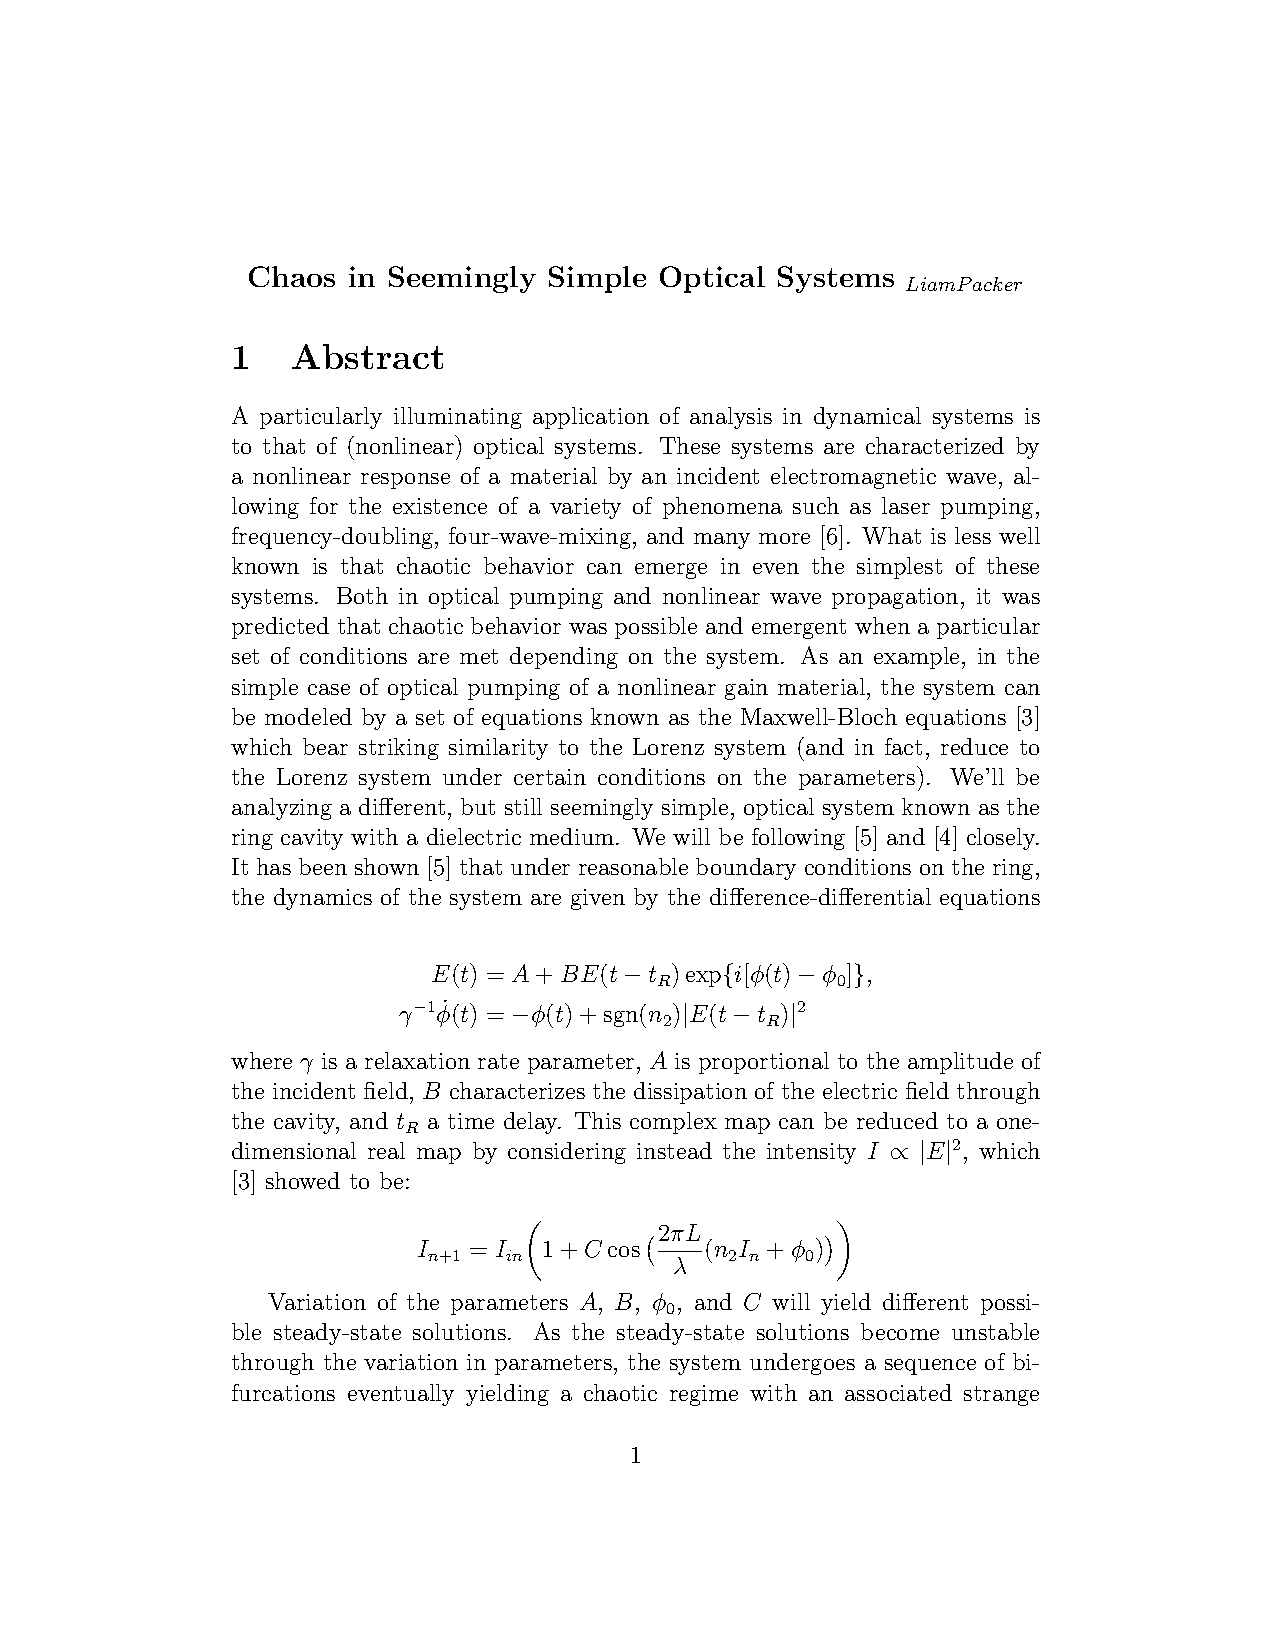
\includegraphics[scale=0.25]{paper.png}}
      \end{figure}
    \end{column}

  \end{columns}
}
\frame{\frametitle{Fractal Dimension}
  \begin{columns}
    \begin{column}{0.5\textwidth}
      \begin{figure}[htbp]
        \centerline{\includegraphics[scale=0.25]{5.0_2.0_0.4_1_minchaos.png}}
      \end{figure}

      \begin{figure}[htbp]
        \centerline{\includegraphics[scale=0.25]{5.0_2.0_0.4_1_minchaos_zoom.png}}
      \end{figure}
    \end{column}
    \begin{column}{0.5\textwidth}
      \begin{figure}[htbp]
        \centerline{\includegraphics[scale=0.3 ]{2.0_0.4_1_correlation.png}}
      \end{figure}
    \end{column}

  \end{columns}

}

\frame{\frametitle{Fractal Dimension}
  \begin{columns}
    \begin{column}{0.5\textwidth}
      \begin{figure}[htbp]
        \centerline{\includegraphics[scale=0.25]{5.0_3.9_0.4_1_paper.png.png}}
      \end{figure}

      \begin{figure}[htbp]
        \centerline{\includegraphics[scale=0.25]{5.0_3.9_0.4_1_paper.png_zoom.png}}
      \end{figure}
    \end{column}
    \begin{column}{0.5\textwidth}
      \begin{figure}[htbp]
        \centerline{\includegraphics[scale=0.3 ]{3.9_0.4_1_correlation.png}}
      \end{figure}
    \end{column}

  \end{columns}

}
\frame{\frametitle{Fractal Dimension}
  \begin{columns}
    \begin{column}{0.5\textwidth}
      \begin{figure}[htbp]
        \centerline{\includegraphics[scale=0.25]{5.0_10.0_0.4_1_paper.png.png}}
      \end{figure}
      \begin{figure}[htbp]
        \centerline{\includegraphics[scale=0.25]{5.0_10.0_0.4_1_paper.png_zoom.png}}
      \end{figure}
    \end{column}

    \begin{column}{0.5\textwidth}
      \begin{figure}[htbp]
        \centerline{\includegraphics[scale=0.3 ]{10.0_0.4_1_correlation.png}}
      \end{figure}
    \end{column}

  \end{columns}

}

% \section{Section no.3}
% \subsection{Tables}
% \frame{\frametitle{Tables}
% \begin{tabular}{|c|c|c|}
    %     \hline
    %     \textbf{Date} & \textbf{Instructor} & \textbf{Title} \\
    %     \hline
    %     WS 04/05 & Sascha Frank & First steps with  \LaTeX  \\
    %     \hline
    %     SS 05 & Sascha Frank & \LaTeX \ Course serial \\
    %     \hline
    %   \end{tabular}}


    %     \frame{\frametitle{Tables with pause}
    %     \begin{tabular}{c c c}
    %     A & B & C \\
    %     \pause
    %     1 & 2 & 3 \\
    %     \pause
    %     A & B & C \\
    %   \end{tabular} }


\section{References}
\frame{\frametitle{References}
  \bibliographystyle{plain}
  \bibliography{refs}

}
\end{document}

%%% Local Variables:
%%% mode: latex
%%% TeX-master: t
%%% End:
